
% ----------------------------------------------------------------------
%  Set the document class
% ----------------------------------------------------------------------
\documentclass[11pt,a4paper,twoside]{article}

% ----------------------------------------------------------------------
% Define external packages, language, margins, fonts and new commands
% ----------------------------------------------------------------------
%\input{preamble} 
\usepackage[utf8]{inputenc}   % <<<<< Linux
\usepackage[english]{babel} % <<<<< English
\usepackage{notoccite}
\usepackage[skip=0.5\baselineskip]{caption}
\hyphenation{GTKWave}
\usepackage{listings}
\usepackage[all]{nowidow}
\usepackage{mathtools}
\usepackage{amsmath}
\usepackage{float}


%blind text
\usepackage{lipsum}

\usepackage{graphicx}
\graphicspath{{./}{../../figlib/}{../mat/}{../sim/}}
\def\FontLn{% 16 pt normal
  \usefont{T1}{phv}{m}{n}\fontsize{16pt}{16pt}\selectfont}
\def\FontLb{% 16 pt bold
  \usefont{T1}{phv}{b}{n}\fontsize{16pt}{16pt}\selectfont}
\def\FontMn{% 14 pt normal
  \usefont{T1}{phv}{m}{n}\fontsize{14pt}{14pt}\selectfont}
\def\FontMb{% 14 pt bold
  \usefont{T1}{phv}{b}{n}\fontsize{14pt}{14pt}\selectfont}
\def\FontSn{% 12 pt normal
  \usefont{T1}{phv}{m}{n}\fontsize{12pt}{12pt}\selectfont}

% Use Arial font as default
%
\renewcommand{\rmdefault}{phv}
\renewcommand{\sfdefault}{phv}
\usepackage{geometry}	
\geometry{verbose,tmargin=2.5cm,bmargin=2.5cm,lmargin=2.5cm,rmargin=2.5cm}

%\usepackage{setspace}
%\renewcommand{\baselinestretch}{1.5}

\usepackage[pdftex]{hyperref} % enhance documents that are to be
                              % output as HTML and PDF
\hypersetup{colorlinks,       % color text of links and anchors,
                              % eliminates borders around links
%            linkcolor=red,    % color for normal internal links
            linkcolor=black,  % color for normal internal links
            anchorcolor=black,% color for anchor text
%            citecolor=green,  % color for bibliographical citations
            citecolor=black,  % color for bibliographical citations
%            filecolor=magenta,% color for URLs which open local files
            filecolor=black,  % color for URLs which open local files
%            menucolor=red,    % color for Acrobat menu items
            menucolor=black,  % color for Acrobat menu items
%            pagecolor=red,    % color for links to other pages
            pagecolor=black,  % color for links to other pages
%            urlcolor=cyan,    % color for linked URLs
            urlcolor=black,   % color for linked URLs
	          bookmarks=true,         % create PDF bookmarks
	          bookmarksopen=false,    % don't expand bookmarks
	          bookmarksnumbered=true, % number bookmarks
	          pdftitle={report},
            pdfauthor={Andre C. Marta},
%            pdfsubject={Thesis Title},
%            pdfkeywords={Thesis Keywords},
            pdfstartview=FitV,
            pdfdisplaydoctitle=true}

\usepackage[numbers,sort&compress]{natbib} % <<<<< References in numbered list [1],[2],...
\usepackage{subcaption} 
\usepackage{mdframed}

%%%%%%%%%%%%%%%%%%%%%%%%%%%%%%%%%%%%%%%%%%%%%%%%%%%%%%%%%%%%%%%%%%%%%%%%
%     Begin Document                                                   %
%%%%%%%%%%%%%%%%%%%%%%%%%%%%%%%%%%%%%%%%%%%%%%%%%%%%%%%%%%%%%%%%%%%%%%%%



\begin{document}

% Set plain page style (no headers, footer with centered page number)
\pagestyle{plain}

% Set roman numbering (i,ii,...) before the start of chapters
%\pagenumbering{roman}

% ----------------------------------------------------------------------
%  Cover page
% ----------------------------------------------------------------------
%%%%%%%%%%%%%%%%%%%%%%%%%%%%%%%%%%%%%%%%%%%%%%%%%%%%%%%%%%%%%%%%%%%%%%%%
%                                                                      %
%     File: frontcover.tex                                             %
%     Tex Master: report.tex                                           %
%                                                                      %
%     Author: Diogo Simões, Júlia Mestre, Rafael Dias                  %
%     Last modified :  21 May 2021                                    %
%                                                                      %
%%%%%%%%%%%%%%%%%%%%%%%%%%%%%%%%%%%%%%%%%%%%%%%%%%%%%%%%%%%%%%%%%%%%%%%%

\thispagestyle {empty}

% IST Logo - Signature A
% parameters: bb=llx lly urx ury (bounding box), width=h_length, height=v_length, angle=angle, scale=factor, clip=true/false, draft=true/false. 
\includegraphics[bb=9.5cm 11cm 0cm 0cm,scale=0.29]{IST_A_CMYK_POS}

\begin{center}
%
% Figure (Image or plot)
\vspace{1.0cm}
% height = 50 mm
%\includegraphics[height=50mm]{Figures/Airbus_A350.jpg}

% Title, author and degree
\vspace{1cm}
{\FontLb Circuit Theory and Electronics Fundamentals} \\ % <<<<< EDIT TITLE
\vspace{1cm}
{\FontSn Department of Physical Engineering, Técnico, University of Lisbon} \\ % <<<<< EDIT COURSE
\vspace{1cm}
{\FontSn Audio Amplifier } \\
\vspace{1cm}
{\FontSn June 3rd, 2021} \\ % <<<<< EDIT DATE (corresponds to date of oral examination)
{\FontSn Diogo Simões, Júlia Mestre, Rafael Dias}
\end{center}



% ----------------------------------------------------------------------
% Dedication page (optional)
% ----------------------------------------------------------------------
%\input{dedication} 
%\cleardoublepage

% ----------------------------------------------------------------------
%  Acknowledgments (optional)
% ----------------------------------------------------------------------
%\input{acknowledgements}
%\cleardoublepage

% ----------------------------------------------------------------------
%  Abstract (both in English and Portuguese)
% ----------------------------------------------------------------------
%\input{resumo} 
%\cleardoublepage

%\input{abstract} 

% ----------------------------------------------------------------------
%  Table of contents, list of tables, list of figures and nomenclature
% ----------------------------------------------------------------------

% Table of contents
%
\tableofcontents

% List of tables
%\addcontentsline{toc}{section}{\listtablename}
%\listoftables

%\cleardoublepage 

% List of figures
%\addcontentsline{toc}{section}{\listfigurename}
%\listoffigures
%\cleardoublepage 

% Set arabic numbering (1,2,...) after preface
%
%\setcounter{page}{1}
%\pagenumbering{arabic}

% ----------------------------------------------------------------------
%  Body
% ----------------------------------------------------------------------

\section{Introduction}
\label{sec:introduction}

% state the learning objective 
The objective of this laboratory assignment is to study a circuit containing a
DC voltage source $V_a$, a current source, $I_d$, a voltage controlled current
source $I_b$, a current controlled voltage source $V_c$ and resistors,
 $R_1$, $R_2$, $R_3$, $R_4$, $R_5$, $R_6$ and $R_7$. The circuit can be seen in Figure \ref{fig:t1}.

\lipsum[1-1]

In Section~\ref{sec:analysis}, a theoretical analysis of the circuit is
presented. In Section~\ref{sec:simulation}, the circuit is analysed by
simulation, and the results are compared to the theoretical results obtained in
Section~\ref{sec:analysis}. The conclusions of this study are outlined in
Section~\ref{sec:conclusion}.

\begin{figure}[h] \centering
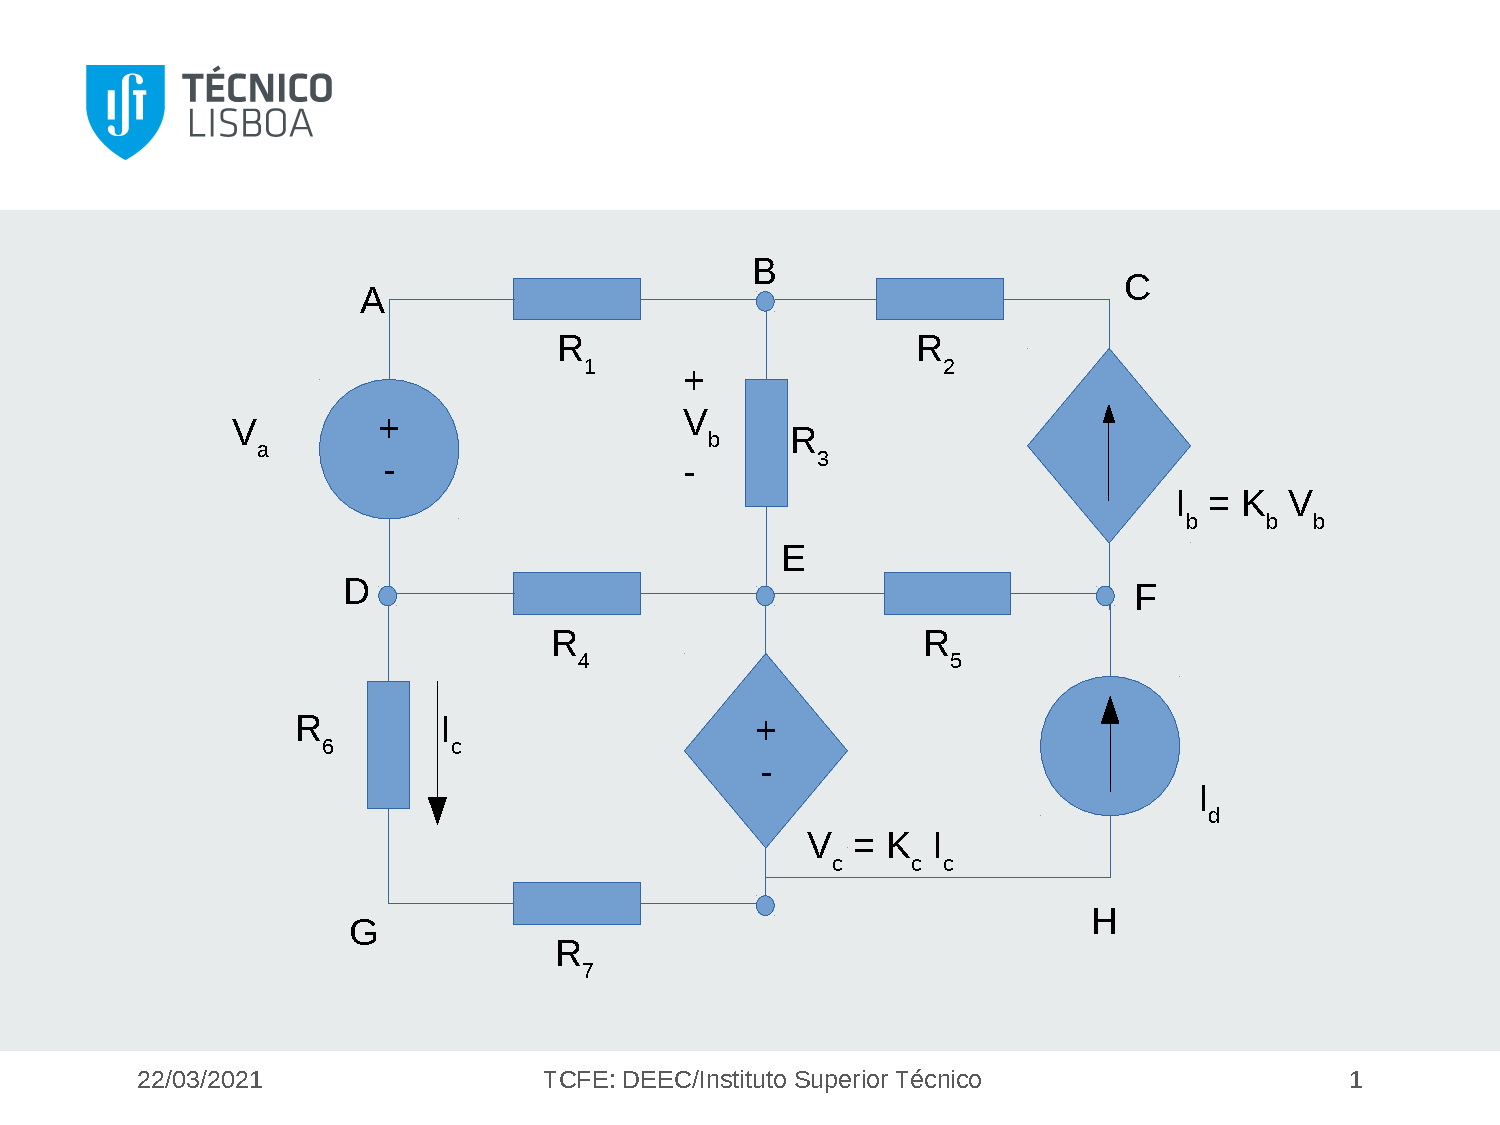
\includegraphics[width=1\linewidth]{t1.pdf}
\caption{Voltage driven serial RC circuit.}
\label{fig:t1}
\end{figure}



\section{Simulation Analysis}
\label{sec:simulation}

We simulated the circuit using frequency analysis, using the supplied model of the OP-AMP:

\begin{table}[H]
\addtolength{\tabcolsep}{-4pt}
\caption{Values of capacitances and resistances for various circuit components}
\vspace{-3mm}
\begin{tabular}{|c|c|c|}
\hline
Vcc & $10.0 V$\\
Vee & $10.0 V$\\
C1 & $220 nF$\\
C2 & $220 nF$\\
R1 & $1000 Ohm$\\
R2 & $500 Ohm$\\
R3 & $100 kOhm$\\
R4 & $1000 Ohm$\\
\hline
\end{tabular}
\label{tab:Components}
\end{table}

\par

We simulate the circuit using frequency analysis and max(vin(t))=1, obtaining the following gain in $v_fin$, which is the gain at the end of the circuit:

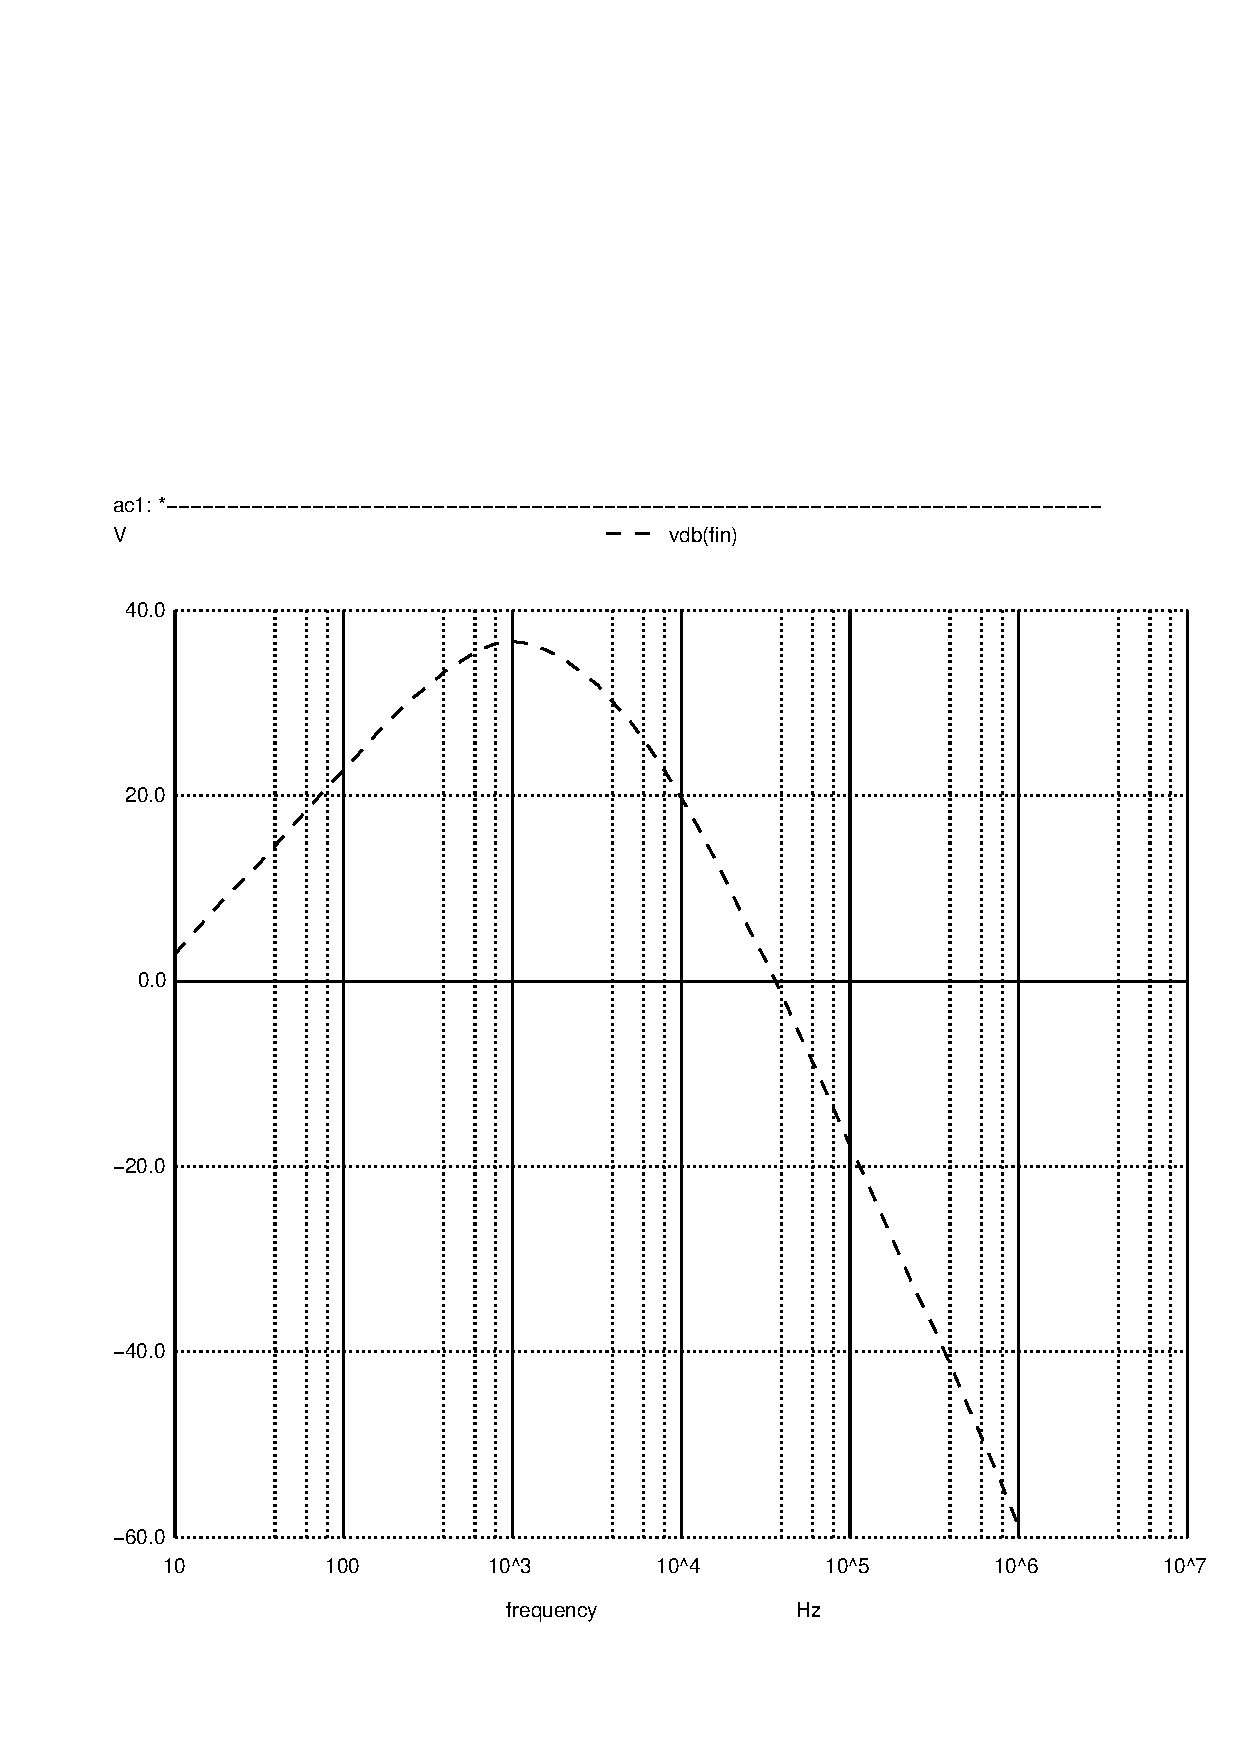
\includegraphics[width=0.8\linewidth]{../sim/vo1f.pdf}

\par

The calculated input impedance is $(990.01+i\cdot 7.32) Ohm$.
A different setup was used to calculate the output impedance which yielded $(-0.09519+i\cdot 7.234) Ohm$.

This circuit has a cost of $113.44$, a maximum gain of $36.55 dB$, central frequency of $1006.5 Hz$.
The calculated merit is therefore $3.9375\cdot 10^{-4}$.


\section{Theoretical Analysis}
\label{sec:analysis}

For the theoretical simulation, we used the dependent voltage source model of the transistors, with Bf1=178.7 and Bf2=227.3.

The bias circuit, which is constituted by $V_c$, $R_{B1}$ and $R_{B2}$, will determine $V_b$.

To simplify the bias circuit, we can ignore the capacitors and make a Thevenin equivalent. This yields:

\begin{equation}
	R_B=\frac{R_{B1} R_{B2}}{R_{B1}+R_{B2}}
\end{equation}

\begin{equation}
	V_{eq}= \frac{R_{B2}}{R_{B1}+R_{B2}} V_{c}
\end{equation}

To calculate the current that passes through the node 8 we know that $I_E= (1+\beta_f)I_B$.

The mesh equation for the bias circuit is $V_{eq} + R_BI_B + V_{Beon} + R_EI_E =0$

Substituting the equation of $I_E$, we now have an expression for $I_B$:
\begin{equation}
	I_{B}= \frac{V_{eq}-V_{ON}}{R_{B}+(1+\beta_F)R_{E}}
\end{equation}

The equation for $I_C$, which is the current that passes trough node 2, is simply $I_C = \beta_F I_B$.

Then, looking at the other mesh, constituted by $R_E, Q_1, R_C$ and$ V_c$, we have the equation:
\begin{equation}
	V_{o}= V_c-R_{C}I_{C}
\end{equation}

By Ohm's Law we also know that $V_E= R_EI_E$ so the voltage between $R_C$ and $R_E$ is: $V_{CE} = V_o - V_E$


We now have all the static voltages and cuurents computed.

For the results of the OP analysis we obtain:

\begin{table}[H]
    \addtolength{\tabcolsep}{-4pt}
    \caption{Some values of the operating point analysis}
    \vspace{-3mm}
    \begin{tabular}{|c|c|}
    \hline
    $I_{b1}$ &  $5.0044e-05$\\
    $I_{e1}$ &  $0.0089929$\\
    $I_{c1}$ &  $0.0089429$  \\ 
    $V_{CE1}$ & $ 2.1578$\\
    $I_{b2}$ &  $3.610556e-04$ \\
    $I_{e2}$ &  $0.082429$\\
    $I_{c2}$ &  $0.082068$\\
    $V_{CE2}$ & $4.4858$\\
    \hline
    \end{tabular}
    \label{tab:OP_mat}
\end{table}

The incremental model of the transistor was used to calculate the input and output impedances, as well as
the gain on both stages of the circuit. The capacitors were modelled as short circuits in this stage. This yields:

\begin{table}[H]
    \addtolength{\tabcolsep}{-4pt}
    \caption{SGains and Impedances}
    \vspace{-3mm}
    \begin{tabular}{|c|c|}
    \hline
    $Z_{i1}$ &  $484.43$\\
    $Z_{o1}$ &  $886.28$\\
    $Z_{i2}$ &  $8598.9$\\
    $Z_{o2}$ &  $0.30217$\\
    $Gain_1$ & $-262.79$\\
    $Gain_2$ &  $0.99195$\\
    $Gain_{Total}$ & $-260.67$\\
    \hline
    \end{tabular}
    \label{tab:Z_mat}
\end{table}

Lastly, the capacitors were re-introduced in order to calculate the gain as a function of the frequency after each stage.
The results are graphed below:

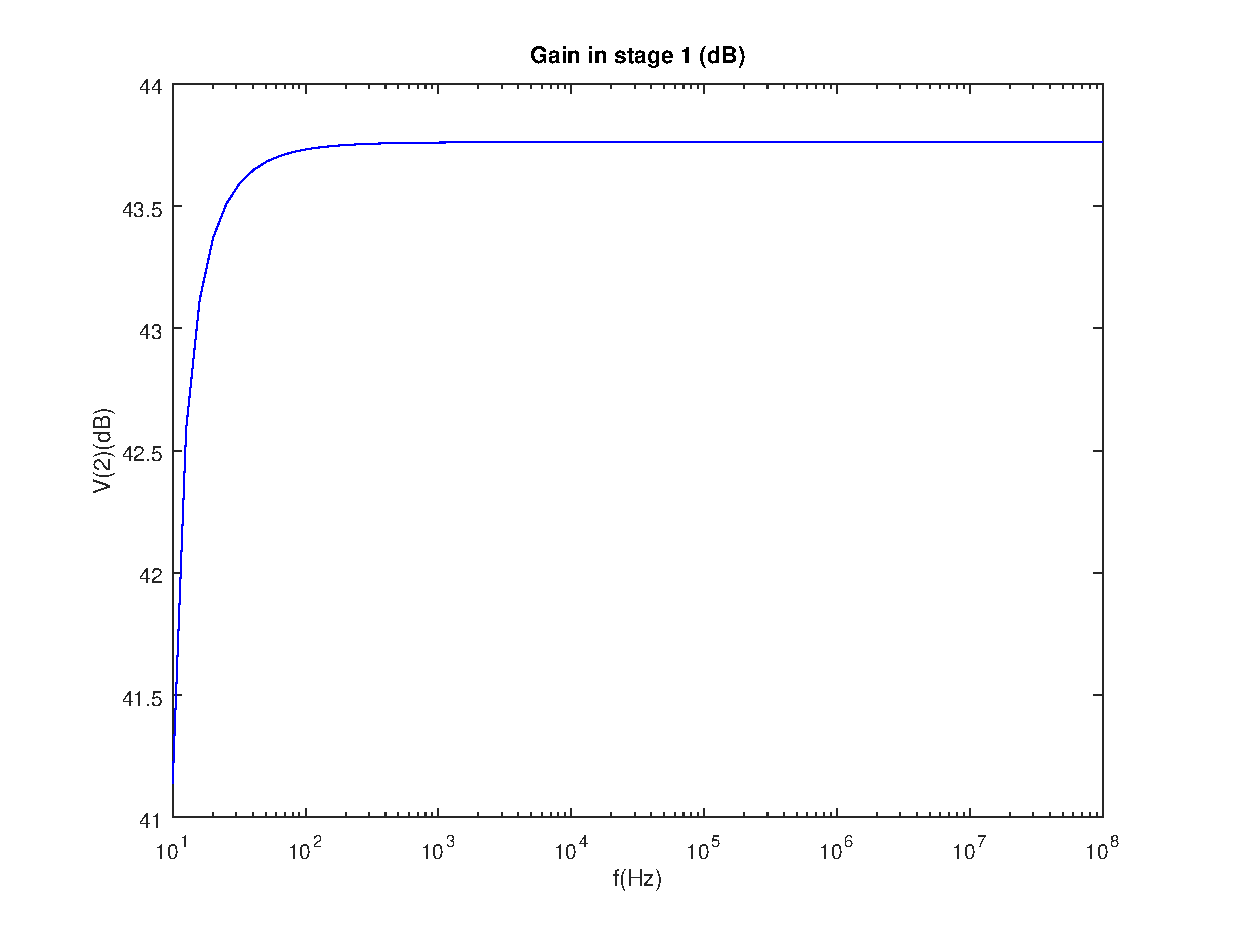
\includegraphics[width=1\linewidth]{vo1.eps}

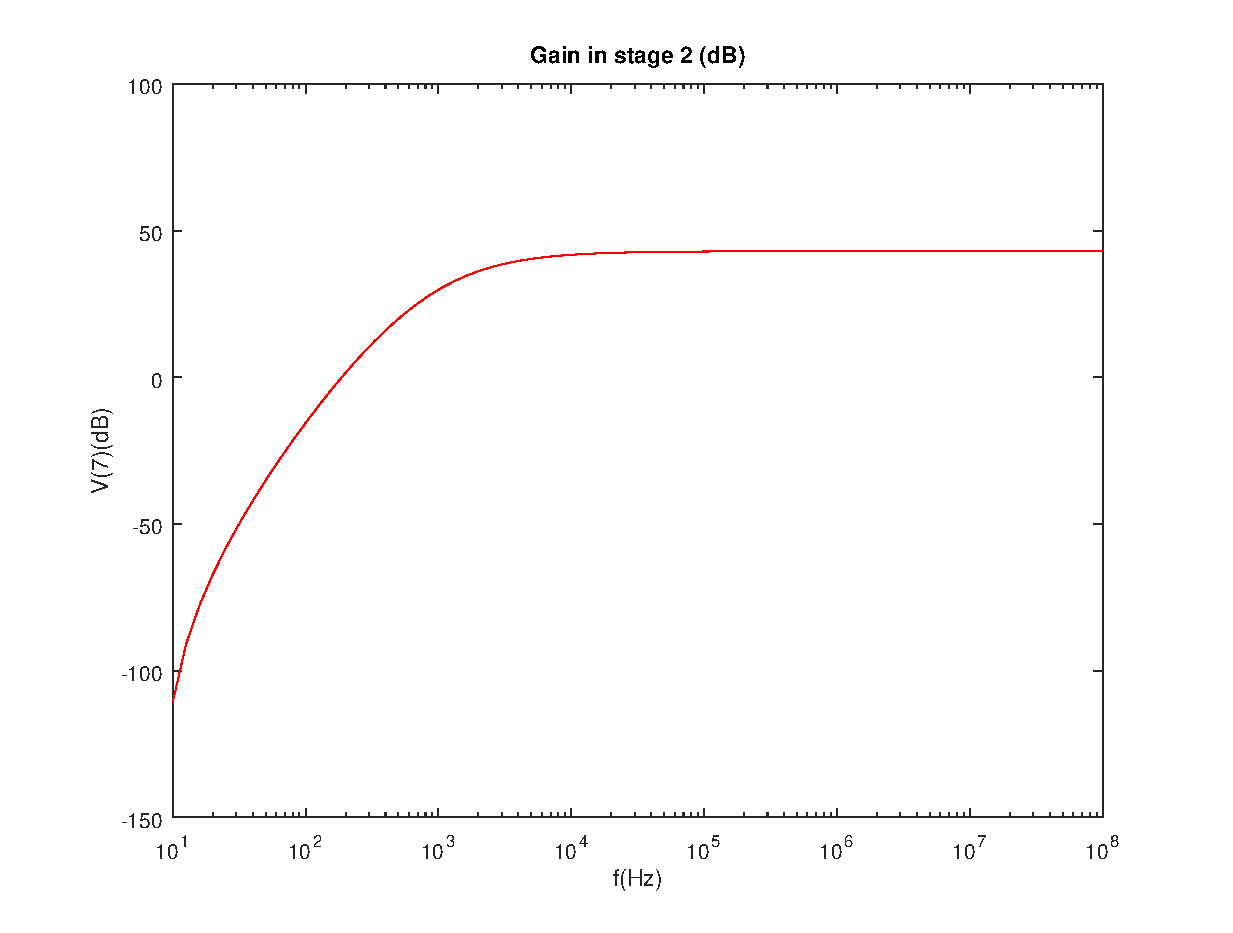
\includegraphics[width=1\linewidth]{vo2.eps}

The lower 3dB cut-off point is at $f=5484.4 Hz$
As we can see, the lower cut-off point is accurrate, but this model does not deal well with the higher cut-off point.


\section{Conclusion}
\label{sec:conclusion}

In this laboratory assignment the objective of analysing a static DC circuit has been
achieved. A static analysis has been performed on the circuit, through both the
node analysis and mesh analysis methods, using the Octave software, and a simulation
was run using ngspice.
The three sets of results all match to 11 decimal places of precision.
The reason for this perfect match is the fact that although this circuit has multiple
components and nodes, all of the components are linear, and no time dependence exists.
The matching of results for the various methods also helps to confirm the accuracy of the equations
used for the theoretical analysis.

%\cleardoublepage

% ----------------------------------------------------------------------
%  Bibliography
% ----------------------------------------------------------------------
%\addcontentsline{toc}{section}{\bibname}
%\bibliographystyle{abbrvunsrtnat} % <<<<< SELECT IF USING REFERENCES BY NUMBER (CITATION ORDER)
%\bibliography{../../../BIBfile.bib}

% ----------------------------------------------------------------------
\end{document}
% ----------------------------------------------------------------------
